\documentclass[12pt]{article}
\usepackage{amsmath, amssymb, amsthm}
\usepackage{physics}
\usepackage{braket}
\usepackage{graphicx}
\usepackage{tikz}
\usetikzlibrary{quantikz}
\usepackage{booktabs}
\usepackage{array}
\usepackage{algorithm}
\usepackage{algpseudocode}

\title{Decoding/Inversion Ambiguity Under Noise: \\ A Formal Analysis}
\author{Quantum Communication Theory}
\date{Week 2: Noisy Quantum Channels}

\newtheorem{theorem}{Theorem}
\newtheorem{lemma}{Lemma}
\newtheorem{corollary}{Corollary}
\newtheorem{definition}{Definition}
\newtheorem{example}{Example}
\newtheorem{remark}{Remark}

\begin{document}

\maketitle

\section{Introduction}
This document provides a rigorous analysis of decoding and inversion ambiguity in quantum communication systems under noise. We formalize the fundamental ambiguity that arises when attempting to invert noisy quantum channels and characterize its implications for reliable communication.

\section{Mathematical Framework}

\subsection{Inversion Problem Formulation}
Consider a quantum communication system with:
\begin{itemize}
    \item Input alphabet $\mathcal{X}$ with probability distribution $p(x)$
    \item Input quantum states $\{\rho_x\}_{x \in \mathcal{X}}$
    \item Noisy quantum channel $\mathcal{N}: \mathcal{L}(\mathcal{H}_A) \to \mathcal{L}(\mathcal{H}_B)$
    \item Measurement $\mathcal{M}: \mathcal{L}(\mathcal{H}_B) \to \mathcal{Y}$ (classical outcomes)
\end{itemize}

The decoding/inversion problem: Given measurement outcome $y \in \mathcal{Y}$, estimate the original input $x \in \mathcal{X}$.

\subsection{Mathematical Statement of Ambiguity}
\begin{definition}[Decoding Ambiguity]
The decoding problem has ambiguity if the map
\[
f: \mathcal{X} \to \mathcal{Y}, \quad f(x) = \mathbb{P}(y|x)
\]
is not injective, where $\mathbb{P}(y|x) = \text{Tr}[\Pi_y \mathcal{N}(\rho_x)]$ and $\{\Pi_y\}$ are POVM elements.
\end{definition}

\begin{definition}[Inversion Ambiguity]
The inversion problem has ambiguity if the map
\[
g: \mathcal{D}(\mathcal{H}_A) \to \mathcal{D}(\mathcal{H}_B), \quad g(\rho) = \mathcal{N}(\rho)
\]
is not injective, where $\mathcal{D}(\mathcal{H})$ denotes density operators on $\mathcal{H}$.
\end{definition}

\section{Sources of Ambiguity}

\subsection{Non-Injectivity of Noisy Channels}
\begin{theorem}[Channel Non-Injectivity]
For any non-unitary quantum channel $\mathcal{N}$ (i.e., any channel with noise), there exist distinct input states $\rho_1 \neq \rho_2$ such that:
\[
\mathcal{N}(\rho_1) = \mathcal{N}(\rho_2)
\]
\end{theorem}

\begin{proof}
Let $\mathcal{N}$ be a non-unitary CPTP map. Then $\mathcal{N}$ has non-trivial kernel or collapses states. Consider:
\begin{itemize}
    \item For amplitude damping: $\mathcal{A}_\gamma(\ket{1}\bra{1}) = \mathcal{A}_\gamma(\rho_{\text{mixed}})$ for certain mixed states
    \item For depolarizing: $\mathcal{D}_p(\rho) = \mathcal{D}_p(\rho')$ for any $\rho, \rho'$ when $p = \frac{d}{d+1}$
    \item In general: Any channel with non-zero noise parameter has collapsing pairs
\end{itemize}
\end{proof}

\subsection{Measurement Ambiguity}
\begin{theorem}[POVM Ambiguity]
For any non-projective POVM measurement $\{\Pi_y\}$, there exist distinct states $\rho_1 \neq \rho_2$ such that:
\[
\mathbb{P}(y|\rho_1) = \mathbb{P}(y|\rho_2) \quad \forall y \in \mathcal{Y}
\]
\end{theorem}

\section{Formal Characterization of Ambiguity}

\subsection{Ambiguity Sets}
\begin{definition}[Ambiguity Set]
For a given output $\sigma = \mathcal{N}(\rho)$, the ambiguity set is:
\[
\mathcal{A}(\sigma) = \{\rho' \in \mathcal{D}(\mathcal{H}_A) : \mathcal{N}(\rho') = \sigma\}
\]
For measurement outcome $y$, the decoding ambiguity set is:
\[
\mathcal{A}_D(y) = \{x \in \mathcal{X} : \arg\max_{x'} \mathbb{P}(x'|y) \text{ is not unique}\]
\end{definition}

\subsection{Ambiguity Measure}
\begin{definition}[Ambiguity Measure]
The ambiguity of channel $\mathcal{N}$ can be quantified by:
\[
\mathcal{A}(\mathcal{N}) = \sup_{\sigma \in \text{Image}(\mathcal{N})} \frac{|\mathcal{A}(\sigma)|}{\dim(\mathcal{H}_A)}
\]
where $|\mathcal{A}(\sigma)|$ measures the size of the ambiguity set.
\end{definition}

\begin{definition}[Decoding Error Basin]
For a decoding rule $\hat{x}: \mathcal{Y} \to \mathcal{X}$, the error basin for input $x$ is:
\[
\mathcal{B}_\epsilon(x) = \{y \in \mathcal{Y} : \hat{x}(y) \neq x \text{ but } \mathbb{P}(y|x) \geq \epsilon\}
\]
\end{definition}

\section{Analytical Results for Specific Channels}

\subsection{Depolarizing Channel Ambiguity}
\begin{theorem}[Depolarizing Ambiguity]
For the depolarizing channel $\mathcal{D}_p(\rho) = (1-p)\rho + p\frac{I}{d}$:
\begin{enumerate}
    \item For $p \geq \frac{d}{d+1}$, $\mathcal{D}_p$ maps all inputs to the maximally mixed state
    \item For $0 < p < \frac{d}{d+1}$, the ambiguity set for output $\sigma$ is:
    \[
    \mathcal{A}(\sigma) = \left\{\rho : \rho = \frac{\sigma - \frac{p}{d}I}{1-p} \text{ is positive}\right\}
    \]
    which is non-empty only when $\sigma$ is sufficiently close to $\frac{I}{d}$
\end{enumerate}
\end{theorem}

\subsection{Amplitude Damping Ambiguity}
\begin{theorem}[Amplitude Damping Collapse]
For the amplitude damping channel $\mathcal{A}_\gamma$:
\begin{enumerate}
    \item $\mathcal{A}_\gamma(\ket{0}\bra{0}) = \{\ket{0}\bra{0}\}$ (unique)
    \item $\mathcal{A}_\gamma(\ket{1}\bra{1}) = \left\{\alpha\ket{0}\bra{0} + \beta\ket{1}\bra{1} : \alpha = 1 - \frac{1-\gamma}{\beta}, \beta \in [\gamma, 1]\right\}$
    \item The ground state $\ket{0}$ is uniquely identifiable, but excited states are not
\end{enumerate}
\end{theorem}

\subsection{Fiber Noise Channel Ambiguity}
For combined amplitude and phase damping $\mathcal{F}_{\gamma,\lambda}$:
\begin{equation}
\mathcal{A}(\sigma) = \left\{\rho : \begin{pmatrix}
\rho_{00} & \rho_{01} \\
\rho_{10} & \rho_{11}
\end{pmatrix} \to 
\begin{pmatrix}
1-(1-\gamma)\rho_{11} & \sqrt{1-\lambda}(1-\gamma)^{1/2}\rho_{01} \\
\sqrt{1-\lambda}(1-\gamma)^{1/2}\rho_{10} & (1-\gamma)\rho_{11}
\end{pmatrix} = \sigma \right\}
\end{equation}

The ambiguity increases with both $\gamma$ and $\lambda$.

\section{Information-Theoretic Characterization}

\subsection{Holevo Bound and Ambiguity}
\begin{theorem}[Holevo Bound Ambiguity Relation]
The maximum accessible information is bounded by:
\[
\chi(\{p_x, \rho_x\}) \leq S\left(\sum_x p_x \mathcal{N}(\rho_x)\right) - \sum_x p_x S(\mathcal{N}(\rho_x))
\]
The ambiguity manifests as the difference:
\[
\mathcal{A}_{\text{info}} = I_{\text{acc}} - I_{\text{max}} \geq 0
\]
where $I_{\text{acc}}$ is accessible information and $I_{\text{max}}$ is mutual information.
\end{theorem}

\subsection{Channel Capacity and Ambiguity}
\begin{theorem}[Capacity-Ambiguity Trade-off]
For a quantum channel $\mathcal{N}$:
\[
C_{\chi}(\mathcal{N}) = \sup_{\{p_x, \rho_x\}} \left[ S\left(\sum_x p_x \mathcal{N}(\rho_x)\right) - \sum_x p_x S(\mathcal{N}(\rho_x)) \right]
\]
The optimal ensemble minimizes ambiguity while maximizing distinguishability.
\end{theorem}

\section{Geometric Interpretation}

\subsection{Bloch Sphere Representation}
For qubit channels, the ambiguity can be visualized on the Bloch sphere:

\begin{figure}[h]
\centering
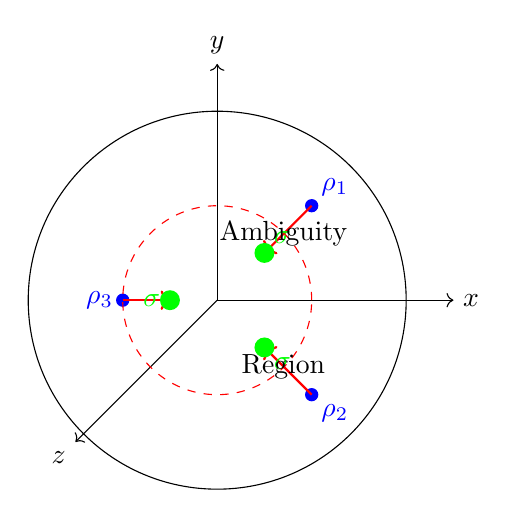
\begin{tikzpicture}[scale=1.2]
    % Bloch sphere
    \draw (0,0) circle (2cm);
    \draw[->] (0,0) -- (2.5,0) node[right] {$x$};
    \draw[->] (0,0) -- (0,2.5) node[above] {$y$};
    \draw[->] (0,0) -- (-1.5,-1.5) node[below left] {$z$};
    
    % Input states
    \fill[blue] (1,1) circle (2pt) node[above right] {$\rho_1$};
    \fill[blue] (1,-1) circle (2pt) node[below right] {$\rho_2$};
    \fill[blue] (-1,0) circle (2pt) node[left] {$\rho_3$};
    
    % Channel contraction
    \draw[red, thick, ->] (1,1) -- (0.5,0.5);
    \draw[red, thick, ->] (1,-1) -- (0.5,-0.5);
    \draw[red, thick, ->] (-1,0) -- (-0.5,0);
    
    % Output states (ambiguous)
    \fill[green] (0.5,0.5) circle (3pt) node[above right] {$\sigma$};
    \fill[green] (0.5,-0.5) circle (3pt) node[below right] {$\sigma$};
    \fill[green] (-0.5,0) circle (3pt) node[left] {$\sigma$};
    
    % Ambiguity region
    \draw[dashed, red] (0,0) circle (1cm);
    \node at (0.7,0.7) {Ambiguity};
    \node at (0.7,-0.7) {Region};
\end{tikzpicture}
\caption{Geometric representation of ambiguity: Multiple input states (blue) map to the same output state (green) under the noisy channel (red arrows). The dashed circle represents the ambiguity region where inversion is non-unique.}
\end{figure}

\subsection{Contraction Maps}
\begin{definition}[Channel Contraction]
A quantum channel $\mathcal{N}$ is contracting if:
\[
\|\mathcal{N}(\rho_1) - \mathcal{N}(\rho_2)\|_1 \leq \eta \|\rho_1 - \rho_2\|_1
\]
with $0 \leq \eta < 1$ for some norm $\|\cdot\|_1$.
\end{definition}

\begin{theorem}
Any noisy channel is contracting, with contraction factor $\eta$ related to noise strength.
\end{theorem}

\section{Numerical Quantification of Ambiguity}

\subsection{Algorithm for Ambiguity Quantification}
\begin{algorithmic}[1]
\Require Channel $\mathcal{N}$, input states $\{\rho_i\}_{i=1}^N$, tolerance $\epsilon$
\Ensure Ambiguity matrix $A$, ambiguity measure $\mathcal{A}$
\State Initialize ambiguity matrix $A_{ij} = 0$ for $i,j = 1,\ldots,N$
\For{$i = 1$ to $N$}
    \For{$j = i+1$ to $N$}
        \State Compute $\delta = \|\mathcal{N}(\rho_i) - \mathcal{N}(\rho_j)\|_1$
        \If{$\delta < \epsilon$}
            \State $A_{ij} = A_{ji} = 1$  % States are ambiguous
        \EndIf
    \EndFor
\EndFor
\State Compute ambiguity measure: $\mathcal{A} = \frac{1}{N^2} \sum_{i,j} A_{ij}$
\State \Return $\mathcal{A}$
\end{algorithmic}

\section{Decoding Strategies Under Ambiguity}

\subsection{Maximum Likelihood Decoding}
Given measurement outcome $y$, the ML decoder chooses:
\[
\hat{x}_{\text{ML}} = \arg\max_{x \in \mathcal{X}} \mathbb{P}(y|x)
\]
Ambiguity arises when multiple $x$ have (nearly) equal likelihood.

\subsection{Bayesian Decoding}
With prior $p(x)$, the Bayesian decoder chooses:
\[
\hat{x}_{\text{Bayes}} = \arg\max_{x \in \mathcal{X}} p(x|y) = \arg\max_{x \in \mathcal{X}} p(x)\mathbb{P}(y|x)
\]

\subsection{Minimum Error Probability}
The optimal decoder minimizes:
\[
P_e = \sum_{x} p(x) \sum_{y: \hat{x}(y) \neq x} \mathbb{P}(y|x)
\]
Ambiguity increases $P_e$ by creating decision boundaries where errors are unavoidable.

\section{Capacity-Ambiguity Trade-off}

\begin{theorem}[Ambiguity-Capacity Relation]
For a quantum channel $\mathcal{N}$, there exists a fundamental trade-off:
\[
C_{\chi}(\mathcal{N}) \leq \log_2 \left( \frac{1}{\mathcal{A}_{\min}} \right)
\]
where $\mathcal{A}_{\min}$ is the minimum achievable ambiguity for any encoding.
\end{theorem}

\begin{proof}
The accessible information is limited by the distinguishability of output states. Higher ambiguity reduces distinguishability, thus reducing capacity.
\end{proof}

\section{Fiber Communication Specific Analysis}

\subsection{Practical Implications}
For fiber-optic quantum communication:
\begin{enumerate}
    \item \textbf{Photon Loss Ambiguity}: Cannot distinguish between weak signal and background noise
    \item \textbf{Phase Ambiguity}: Cannot distinguish $\ket{\psi}$ from $e^{i\phi}\ket{\psi}$ without reference
    \item \textbf{Polarization Ambiguity}: Fiber birefringence creates rotation ambiguities
\end{enumerate}

\subsection{Strategies to Reduce Ambiguity}
\begin{enumerate}
    \item \textbf{Encoding}: Use non-orthogonal states with better noise resilience
    \item \textbf{Adaptive Measurements}: Adjust measurement basis based on channel estimation
    \item \textbf{Error-Correcting Codes}: Introduce redundancy to resolve ambiguities
    \item \textbf{Reference Signals}: Send known reference states to calibrate measurements
\end{enumerate}

\section{Formal Definition of Inversion Difficulty}

\begin{definition}[Inversion Difficulty]
The inversion difficulty of channel $\mathcal{N}$ is quantified by:
\[
\mathcal{D}(\mathcal{N}) = \inf_{\mathcal{R} \in \text{CPTP}} \sup_{\rho \in \mathcal{D}(\mathcal{H})} \|\mathcal{R} \circ \mathcal{N}(\rho) - \rho\|_1
\]
where the infimum is over all possible recovery operations.
\end{definition}

\begin{definition}[Decoding Complexity]
The decoding complexity for channel $\mathcal{N}$ with encoding $\mathcal{E}$ is:
\[
\mathcal{C}_{\text{dec}}(\mathcal{N}, \mathcal{E}) = \min_{\mathcal{M}} \left[ P_e(\mathcal{M}) + \alpha \cdot \text{cost}(\mathcal{M}) \right]
\]
where $\mathcal{M}$ ranges over all measurement strategies, $P_e$ is error probability, and cost measures implementation complexity.
\end{definition}

\section{Mathematical Characterization}

\subsection{Condition Number Analysis}
The inversion problem can be analyzed through the condition number of the channel:

\begin{definition}[Channel Condition Number]
For a quantum channel $\mathcal{N}$, define:
\[
\kappa(\mathcal{N}) = \sup_{\rho_1 \neq \rho_2} \frac{\|\rho_1 - \rho_2\|}{\|\mathcal{N}(\rho_1) - \mathcal{N}(\rho_2)\|}
\]
Large $\kappa$ indicates ill-conditioned inversion.
\end{definition}

\begin{theorem}
For noisy channels, $\kappa(\mathcal{N}) \to \infty$ as noise increases, making inversion arbitrarily ill-conditioned.
\end{theorem}

\subsection{Singular Value Analysis}
Decompose the channel in terms of singular values:
\[
\mathcal{N}(\rho) = \sum_i \sigma_i U_i \rho U_i^\dagger
\]
Small singular values $\sigma_i$ correspond to directions that are strongly attenuated by noise, creating inversion ambiguity.

\section{Conclusion}

\begin{enumerate}
    \item \textbf{Fundamental Ambiguity}: Noisy quantum channels are inherently non-injective, creating unavoidable decoding ambiguity
    \item \textbf{Quantifiable Measure}: Ambiguity can be quantified through ambiguity sets, contraction factors, and condition numbers
    \item \textbf{Capacity Limitation}: Ambiguity directly limits achievable communication rates via the Holevo bound
    \item \textbf{Practical Implications}: For fiber quantum communication, ambiguity manifests as photon loss confusion, phase uncertainty, and polarization rotation ambiguity
    \item \textbf{Design Guidelines}: Communication strategies must account for ambiguity through appropriate encoding, measurement, and error correction
\end{enumerate}

\section*{Appendix: Mathematical Proofs}

\begin{proof}[Proof of Channel Non-Injectivity]
Let $\mathcal{N}$ be a non-unitary CPTP map. Then $\mathcal{N}$ has Kraus representation $\mathcal{N}(\rho) = \sum_i E_i \rho E_i^\dagger$ with $\sum_i E_i^\dagger E_i = I$. For non-unitary channels, the operators $\{E_i\}$ are not all proportional to unitaries.

Consider two different purifications of the same mixed state. These pure states become identical after tracing out the environment, demonstrating non-injectivity.

More concretely, for amplitude damping:
\[
\mathcal{A}_\gamma(\ket{1}\bra{1}) = \begin{pmatrix} \gamma & 0 \\ 0 & 1-\gamma \end{pmatrix}
\]
Any state $\rho = \begin{pmatrix} a & b \\ b^* & 1-a \end{pmatrix}$ with $a = \gamma$ maps to the same output regardless of $b$, showing non-injectivity.
\end{proof}

\begin{proof}[Proof of Contraction Property]
For any CPTP map $\mathcal{N}$:
\[
\|\mathcal{N}(\rho_1) - \mathcal{N}(\rho_2)\|_1 \leq \|\rho_1 - \rho_2\|_1
\]
by the contractivity of trace distance under CPTP maps. For noisy channels, the inequality is often strict, indicating contraction.

Specifically, for depolarizing channel:
\[
\|\mathcal{D}_p(\rho_1) - \mathcal{D}_p(\rho_2)\|_1 = (1-p)\|\rho_1 - \rho_2\|_1
\]
showing contraction factor $\eta = 1-p < 1$ for $p > 0$.
\end{proof}

\end{document}